\section{Hardware implementation\label{section-hardware}}

\subsection{Restrictions}

Since the design will be synthesized using a 0.13 $\mu m$ low leakage library by Faraday Corporation \cite{cell-databook}, we first take a look at which cells take up the largest area. A listing is given in \reftbl{table-cells}. It's clear that the usage of both registers and multiplexors should be kept to a minimum.

\begin{table}[h]
	\caption[Area of cells in an ASIC circuit]{Area of cells in an ASIC circuit (0.13 $\mu m$ low leakage technology by Faraday Corporation \cite{cell-databook})}
	\label{table-cells}

	\centering
	\begin{tabular}{lr}
		\toprule
		Cell							& Area $\left[\frac{\text{gate}}{\text{bit}}\right]$\\
		\midrule
		D flip-flop (reset)		& 6\\
		D flip-flop (no reset)	& 5,5\\
		D latch						& 4,25\\
		3 input MUX					& 4\\
		2 input XOR					& 3,75\\
		2 input MUX					& 2,25\\
		2 input NAND				& 1\\
		NOT							& 0,75\\
		\bottomrule
	\end{tabular}
\end{table}

\subsection{Arithmetic core}

The core of the implementation is the MALU \cite{sakiyama, batina-pkc}, which can calculate the sum of two elements $a, b \in \mathbb{F}_{2^m}$ as well as a modulo operation. Its design is shown in \reffig{figure-malu}. For the given parameters we need 167 XOR gates to construct this circuit.

\begin{figure}[h]
	\centering
		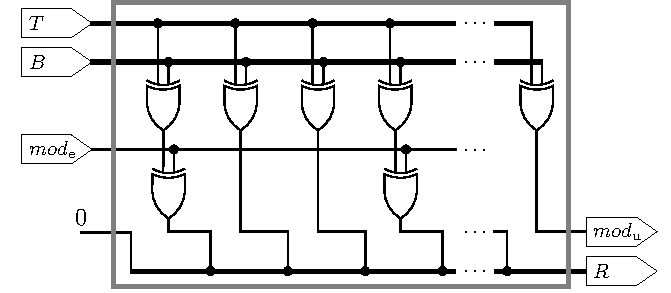
\includegraphics[width=3.5in]{malu-optimized}
		\caption{Arithmetic core for addition and modular reduction in $\mathbb{F}_{2^m}$\label{figure-malu}}
\end{figure}

Building on this, we construct a wrapper that allows multiplication in $\mathbb{F}_{2^m}$ as well. The result of a multiplication is calculated using the `shift-and-add' technique. To be able to do this, we need one extra register $T$ to store temporary results. The circuit and its control logic is shown in respectively \reffig{figure-gf2m} and \reffig{figure-gf2m-logic}. Note that when executing a multiplication, the input $A$ needs to be shifted to the left by one bit every clock cycle. This task is left up to whatever circuit implements this one. Instead of one MALU, multiple ones can be daisy-chained together to speed up the calculation of a multiplication.

\begin{figure}[h]
	\centering
		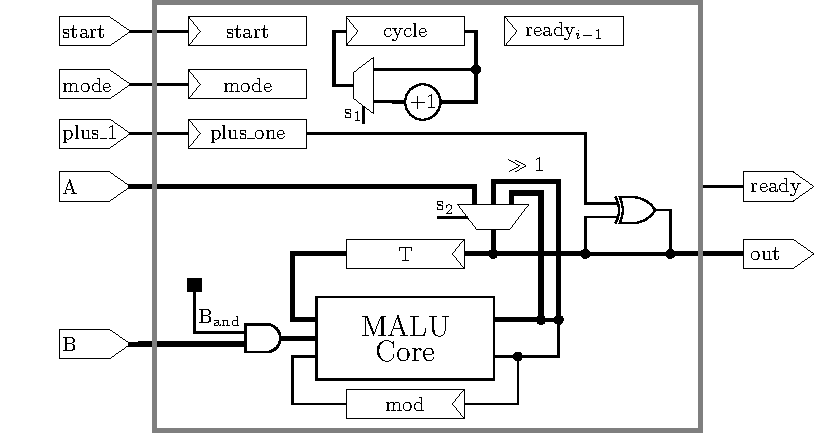
\includegraphics[width=3.5in]{wrapper-gf2m}
		\caption{$\mathbb{F}_{2^m}$ arithmetic wrapper circuit\label{figure-gf2m}}
\end{figure}

\begin{figure}[h]
	\centering
		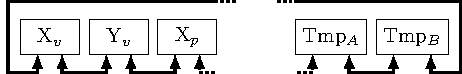
\includegraphics[width=3.5in]{wrapper-gf2m-logica}
		\caption{$\mathbb{F}_{2^m}$ arithmetic wrapper circuit - Control logic\label{figure-gf2m-logic}}
\end{figure}

\subsection{Controller for Miller's algorithm}

Finally, we create a controller that contains memory and the aforementioned circuit. The general design is shown in \reffig{figure-controller}. The \emph{next} input is used to signal that there's either a new coordinate available at the input or that the next part of the result should be put on the output.

\begin{figure}[h]
	\centering
		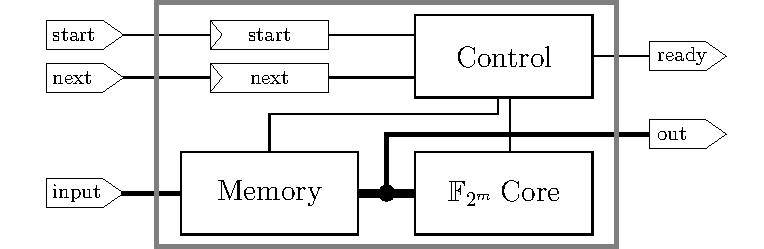
\includegraphics[width=3.5in]{controller-miller}
		\caption{Controller for Miller's algorithm\label{figure-controller}}
\end{figure}

Before we can correctly asses the merits of various memory designs, we need to know how many registers we need. After writing out every calculation in Miller's algorithm, the minimum number of registers was found to be fifteen registers. This excludes the one register in the $\mathbb{F}_{2^m}$ wrapper. 

The basis for the memory is a compact design by Lee and Verbauwhede \cite{lee}. They propose a unidirectional circular shift register file in which the first two registers are connected to the arithmetic core. Furthermore, it's possible to swap the contents of the first two registers. While this design is certainly about as small as it gets, using it in a register file with fifteen registers is not really feasible for a low power design. We will try to prove this in the next few paragraphs by calculating the average number of write operations $\overline{w}$ that have to be executed before every arithmetic operation. This number is directly proportional to the energy consumed.

The numbers that follow are rough averages and should be interpreted as such. Assume the size of the register file is $n$. First, calculate the average distance $\overline{r}$ between two registers by dividing the sum of possible distances $s$ by the number of possible combinations $c$:
\begin{displaymath}\begin{aligned}
	s	&= \sum_{i = 1}^{n - 1} \sum_{j = i + 1}^n (j - i - 1)
		&\qquad c	&= \sum_{i = 0}^{n - 1} i\\
		&= \frac{n \cdot (n - 1) \cdot (n - 2)}{6}
		&	&= n \cdot \frac{n - 1}{2},\\
\end{aligned}\end{displaymath}
thus:
\begin{displaymath}\overline{r}	= \frac{n - 2}{3}.\end{displaymath}
Now the average number of write operations $\overline{w}$, which have to be executed before every arithmetic operation, can be calculated. First, calculate the average number of cycles it takes to move the content of two registers to register one and two. This is equal to $\overline{r}$ times $n$. Multiplying this by the number of writes that have to be executed each cycle, gives us $\overline w$. Since shifts are only possible in one direction, every such shift demands $n$ write operations. The result is
\begin{displaymath}
	\overline{w} = O ( n^3 ).
\end{displaymath}

Now we will calculate $\overline{w}$ for a register file in which shifts in both directions are possible. Again, we first calculate:
\begin{displaymath}\begin{aligned}
	\overline{r}	&= \frac{1}{n} \cdot \sum_{i = 1}^{n} \textsf{min}(j - 1, n - j + 1)\\
						&= \frac{n - 1}{4}.
\end{aligned}\end{displaymath}
In this case, the content of non-adjacent registers can be swapped independently. Thus, the average number of clock cycles will be equal to the average distance to the start of the register file: $\frac{n}{2}$. Every swap operation requires two write operations and there's two values to be moved to the front of the register file. With all this in mind, we find
\begin{displaymath}\overline{w} = O(n).\end{displaymath}

Even though the resulting register file will be larger due to the addition of muxes, we favor it due to its lower energy consumption. A diagram of the design is shown in \reffig{figure-regs}.

\begin{figure}[h]
	\centering
		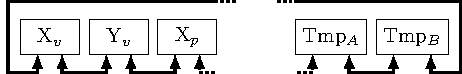
\includegraphics[width=3.5in]{geheugen-circ-optimized}
		\caption{Register file design\label{figure-regs}}
\end{figure}

Notice that since the first register is connected to the arithmetic core's input $A$, it needs to be able to store its own value shifted to the left. Thus register one will require a larger mux.

Using this register file design, the FSM to control the circuit consists of 553 states. Most of these are due to register contents having to be swapped around.

\subsection{Optimizations}

Since the arithmetic core is already very small, we will focus our optimization efforts on the register file.

First of all, the reset inputs of as many registers as possible are removed. As can be seen in \reftbl{table-cells}, this will save 8.5\% area compared to a register with resets.

Clock gating is implemented for every register using the circuit shown in \reffig{figure-cg}. Compared to a clock gating circuit which ANDs the clock and enable signal together, this one has the benefit of keeping the clock input high while idle. As shown in \cite{mueller} this reduces power consumption. It can be argued though that, for this register file design, power saving improvements will probably be negligible.

\begin{figure}[h]
	\centering
		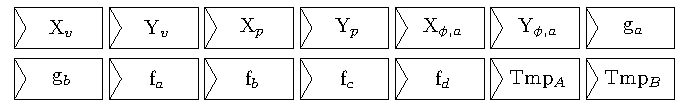
\includegraphics[width=3.5in]{cg-low-power}
		\caption{Clock gating circuit\label{figure-cg}}
\end{figure}
